% HopkinsonSimulator report: the theory of the simulator and of the Bussac wave separation.
%
% The layout comes from reports/template/hopkinson_report.sty (a copy of the layout of the sigmaSPH
% technical reports), which the Makefile finds through TEXINPUTS. The figures are made by
% make_figures.py in this folder with the code of the two programs.
\documentclass[11pt,a4paper,numbers=noenddot,abstract=true]{scrartcl}
\usepackage{hopkinson_report}
\usepackage[capitalise,noabbrev]{cleveref}
\usetikzlibrary{decorations.pathmorphing}
% written by make_figures.py; do not edit
\newcommand{\shpbValid}{812}
\newcommand{\shpbFmax}{345}
\newcommand{\shpbWaveErr}{1.1 \cdot 10^{-2}}
\newcommand{\shpbForceErr}{3.0 \cdot 10^{-2}}
\newcommand{\shpbImbSep}{0.1}
\newcommand{\shpbImbTrue}{0.0}
\newcommand{\shtbValid}{1812}
\newcommand{\shtbFmax}{345}
\newcommand{\shtbWaveErr}{5.9 \cdot 10^{-3}}
\newcommand{\shtbForceErr}{2.2 \cdot 10^{-2}}
\newcommand{\shtbImbSep}{0.2}
\newcommand{\shtbImbTrue}{0.0}
   % numbers of the worked examples, written by make_figures.py
\graphicspath{{figures/}}
\urlstyle{tt}
\newcommand{\code}[1]{\texttt{\detokenize{#1}}}
\DeclareMathOperator{\Imag}{Im}
\DeclareMathOperator{\cov}{cov}

\reporttitle{Theory of the Hopkinson bar simulator\\ and of the Bussac wave separation}
\reportshorttitle{Theory of HopkinsonSimulator}
\reportsubtitle{The spectral propagator, the bar models, and the least-squares separation of waves}
\reportauthor{Georg C. Ganzenmüller}
\reportdate{10 November 2026}

\begin{document}
\makereporttitle

\begin{abstract}
This report describes the methods behind the two programs of HopkinsonSimulator. The simulator produces the
strain-gauge records of a split Hopkinson bar test together with the exact waves at the two bar--specimen
interfaces. It does not discretise the bars. It moves known time histories along them with a spectral
propagator, the factor $e^{-ik(\omega)x}$ of each frequency, and couples the bars to a time-domain specimen model
by a fixed-point iteration. The report explains why this suits the long, slender, uniform and linear bars of a
Hopkinson test better than a finite-difference or finite-element model: the propagation is exact for the chosen
bar model, its cost does not depend on the bar length, lateral inertia and three-dimensional dispersion enter
only through $k(\omega)$, and the stored waves are exactly the cause of the records. It states the three bar
models: the one-dimensional wave equation, the Love rod, and the first mode of the Pochhammer--Chree solution.
The analysis separates the gauge records by the method of Bussac, Collet, Gary and Othman. The report derives it
first for two gauges, where it is a system of two equations in two unknowns that is singular at the frequencies
at which the gauge spacing is a whole number of half wavelengths, and shows how the Laplace damping removes these
singularities. It then generalises the method to $N$ gauges as a least-squares problem, and shows that its
solution is the most likely pair of waves when the gauges carry independent noise of equal variance. The
conditions of this interpretation are stated. Two worked examples, a split Hopkinson pressure bar and a split
Hopkinson tension bar, show the simulated gauge records, the separated waves against the simulated ones, and the
force balance of the specimen. The examples show that the method works on two cases; they are not a study of its
accuracy.
\end{abstract}
\clearpage

\tableofcontents
\clearpage

% =====================================================================================================
\section{Introduction}
\label{sec:introduction}

This report describes the methods behind the two programs of HopkinsonSimulator.
\Cref{sec:propagator,sec:why,sec:models} treat the simulator: how waves are moved along the bars with a spectral
propagator instead of a discretised bar, why this suits the geometry of a Hopkinson bar, and the three bar models.
\Cref{sec:problem,sec:twogauges,sec:ngauges,sec:likely,sec:implementation} treat the Bussac wave separation used
by the analysis: first with two strain gauges, where it is a system of two equations in two unknowns, then with
$N$ gauges, where it becomes a least-squares problem whose solution is the most likely one under a stated noise
model. \Cref{sec:examples} applies both programs to two worked examples, a pressure bar and a tension bar.

The README of the project describes how to run the programs and the format of their files. This report describes
the methods, and names the functions of the code where it helps.

\subsection{Notation and conventions}
\label{sec:notation}

\Cref{tab:notation} defines the symbols. The Fourier transform follows numpy:
$X(\omega) = \sum_n x(t_n)\, e^{-i\omega t_n}$. A component of frequency $\omega$ therefore varies in time as
$e^{+i\omega t}$, and a wave that travels in the $+x$ direction has the form $e^{i(\omega t - kx)}$. Moving such a
wave a distance $s \ge 0$ in its own direction of travel multiplies its spectrum by
\begin{equation}
  H(\omega; s) = e^{-i k(\omega) s}.
  \label{eq:propagator}
\end{equation}
For real $k > 0$ this is a pure delay of each component by $s / c(\omega)$. For complex $k$ with $\Imag k < 0$ the
component also decays, by $e^{-\kappa s}$ with $\kappa = -\Imag k$.

\begin{table}[htbp]
\centering
\caption{Symbols used in this report.}
\label{tab:notation}
\begin{tabularx}{\textwidth}{lX}
\toprule
symbol & meaning \\
\midrule
$x$ & distance along a bar, measured from the bar--specimen interface into the bar (local coordinate) \\
$t$ & time \\
$\omega$, $f$ & angular frequency and frequency, $\omega = 2\pi f$ \\
$k(\omega)$ & wavenumber of the bar model \\
$c(\omega) = \omega / k$ & phase velocity; $c_g = d\omega / dk$ is the group velocity \\
$E$, $\rho$, $\nu$ & Young's modulus, density and Poisson's ratio of a bar \\
$a$, $A$ & bar radius and cross-section area \\
$c_0 = \sqrt{E/\rho}$ & bar wave speed of the one-dimensional wave equation \\
$\varepsilon$ & axial strain, positive in tension \\
$N$ & axial force, positive in tension \\
$v$ & particle velocity, positive along the global axis, which points from the input bar to the output bar \\
\bottomrule
\end{tabularx}
\end{table}

% =====================================================================================================
\section{The spectral propagator}
\label{sec:propagator}

\subsection{What is computed}

A Hopkinson bar test has an input bar, a short specimen and an output bar, all on one axis. The loading differs
between the three setups of the project:
\begin{itemize}
  \item \emph{split Hopkinson pressure bar (SHPB):} a strain pulse is sent into the input bar;
  \item \emph{direct impact:} the input bar itself is the projectile;
  \item \emph{split Hopkinson tension bar (SHTB):} a tubular striker hits a flange at the far end of the input bar.
\end{itemize}
Strain gauges on both bars record the strain at a few points.

The simulator has to produce two things: the gauge records, and the exact waves at the two bar--specimen
interfaces that caused them. The second is what makes the simulator useful as a reference. A wave-separation
method sees only the records, and its result can be compared with the stored interface waves.

At each interface there are two strain waves: $a(t)$, the incoming wave, which travels towards the specimen, and
$b(t)$, the outgoing wave, which travels away from it. The interface strain is $a + b$. The unknowns of the
simulator are these four time histories, $a_1, b_1$ on the input bar and $a_2, b_2$ on the output bar. The bars
themselves are not divided into elements or cells.

\subsection{A uniform linear bar acts as a filter}

The bars are homogeneous and linear, and their cross-section does not change along their length. Two
consequences follow. First, the strain anywhere in a bar is the sum of two waves that travel in opposite
directions, because the bar has no internal source. Second, each frequency component travels independently of
the others. A wave known as a time history at one position is therefore known at every other position: its
spectrum is multiplied by $H(\omega; s)$, and the inverse transform gives its time history there. The whole effect
of the bar, including its dispersion, is contained in the single function $k(\omega)$. \Cref{sec:shift} derives this factor from the time shift of a
wave in the one-dimensional bar.

The simulator uses this directly. The incident pulse of the SHPB is prescribed at a source position at distance
$d$ from the interface; the incoming wave at the interface is then
$a_1 = \mathcal{F}^{-1}\bigl[H(\omega; d)\, \mathcal{F}[\varepsilon_\mathrm{ref}]\bigr]$. An outgoing wave $b$
travels to the free far end of a bar of length $L$ and back. It returns to the interface as the incoming wave
$-\mathcal{F}^{-1}\bigl[H(\omega; 2L)\, \mathcal{F}[b]\bigr]$; the sign change is the reflection at a free end,
where the stress vanishes.

A strain gauge of length $L_g$ measures the strain averaged over its length. For a wave $e^{-ikx}$, the average
over $[x - L_g/2,\, x + L_g/2]$ is the point value multiplied by
\begin{equation}
  G(\omega) = \frac{\sin(k L_g / 2)}{k L_g / 2},
  \label{eq:gauge}
\end{equation}
which also holds for complex $k$. The gauge records are therefore computed exactly, by a further factor in the
frequency domain (function \code{gauge_average_factor}).

\subsection{Particle velocity and force}

Particle velocity and force follow from the strain of a single wave with operators of the same kind. For a wave
that travels in the $\pm x$ direction,
\begin{equation}
  v = \mp \frac{\omega}{k}\, \varepsilon, \qquad
  N_E = A E\, \varepsilon, \qquad
  N_\mathrm{eff} = A \rho \left(\frac{\omega}{k}\right)^{\!2} \varepsilon.
  \label{eq:operators}
\end{equation}
For the one-dimensional wave equation $\omega / k = c_0$, and both forces are equal. For the Love rod,
$N_\mathrm{eff}$ is exactly the force of the Love effective stress, which includes the lateral inertia. For the
Kelvin--Voigt bar, $N_\mathrm{eff} = A E (\varepsilon + \tau \dot\varepsilon)$. These operators are the functions
\code{wave_velocity} and \code{force_eff}.

\subsection{Discrete transforms}

The fast Fourier transform treats a record as one period of a periodic signal, so a delayed wave would wrap
around from the end of the record to its start. The simulator prevents this in two ways. The records are padded
with zeros to a length of \code{pad_factor} times the record (8 in the examples). And frequency components whose
group delay over the longest path is longer than the padding are excluded, because they would arrive after the
end of the record anyway. This matters only for the Love rod close to its cut-off, where $c_g \to 0$.

The excluded band is evaluated for one fixed distance, the longest path in the simulation. This keeps the
propagators exactly composable, $H(s_1)\, H(s_2) = H(s_1 + s_2)$, including the excluded band; a test checks this
to $10^{-11}$.

The frequency-domain operators for velocity and force act on the whole record. On a record that ends while waves
are still present, they would ring near its end. The simulation therefore runs for \code{truth_margin} beyond the
stored record, and the result is cropped.

\subsection{Coupling with the specimen}

The specimen is nonlinear (elastic--plastic, with unilateral contact in the pressure setups) and is solved in the
time domain. It sees each bar through the relations of the non-dispersive bar: for the input bar,
$N_1 = E_1 A_1 (a_1 + b_1)$ and $v_1 = c_{0,1} (-a_1 + b_1)$, and correspondingly for the output bar. Given the
incoming waves $a_1$ and $a_2$, the specimen model returns the interface force, and force balance gives the
outgoing waves,
\begin{equation}
  b = \frac{N}{E A} - a.
\end{equation}
This coupling is not at the level of the dispersive bar models. It affects how realistic the specimen response is
for a dispersive bar. It does not affect the consistency between the stored waves and the gauge records, because
those are computed from the same $a$ and $b$ afterwards.

The incoming waves depend on the outgoing ones through the far-end echoes, and the outgoing ones depend on the
incoming ones through the specimen. The simulator resolves this with a fixed-point iteration. Each pass forms the
incoming waves from the loading and from the echoes of the outgoing waves of the previous pass, solves the
specimen, and obtains new outgoing waves. An echo needs at least one round trip in a bar to return, so each pass
makes the solution exact for one more round trip. The iteration stops when the outgoing waves change by less than
$10^{-8}$ relative between passes; this takes 5 to 7 passes for the example cases with the Love rod.

The specimen is integrated on a finer time grid than the records (\code{n_sub} substeps per sample). The incoming
waves are interpolated onto this grid by band-limited (trigonometric) interpolation, which is exact for the
sampled band.

\subsection{The loading in the three setups}

\paragraph{SHPB.} The prescribed pulse $\varepsilon_\mathrm{ref}$ is propagated from the source to the interface.

\paragraph{Direct impact.} The input bar moves at $v_0$ with zero strain and hits the specimen. For the specimen
this is the same as a bar at rest that receives an additional step wave $-v_0 / (2 c_0)$. The gauges see only the
strain waves, and $v_0$ is added to the input-bar velocity.

\paragraph{SHTB.} The loading end, with a rigid flange and a striker that can separate from it and hit it again,
is solved in the time domain in the same way as the specimen, and is coupled to the input bar through the same
iteration.

% =====================================================================================================
\section{Why a spectral propagator rather than a discretised bar}
\label{sec:why}

A finite-difference or finite-element model divides the bar into cells and integrates the field in time. The
spectral propagator never represents the field along the bar; it moves known time histories from one position to
another. For a Hopkinson bar this has five advantages.

\paragraph{The propagation is exact for the chosen bar model.} The factor $e^{-ikx}$ is the exact solution of the
bar model for each frequency. A discretised bar has a numerical dispersion error: the phase velocity of the scheme
differs slightly from the true one, the difference depends on frequency and on the cell size, and its effect
accumulates with the distance travelled. In the 1~ms record of the SHPB example, waves travel up to
$c_0 \times 1~\mathrm{ms} \approx 5$~m (from the source to the interface, then towards the far end). The sharp
rise of the incident pulse contains components above 200~kHz, whose wavelength in the aluminium bar is 25~mm or
less, so the path is about two hundred wavelengths long. Over $D / \lambda$ wavelengths, a relative error
$\delta c / c$ in the phase velocity shifts the phase by $2\pi\, (D / \lambda)\, \delta c / c$. To keep this below
0.01~rad over 200 wavelengths, the scheme would need $\delta c / c < 8 \cdot 10^{-6}$ at these frequencies. The
simulator is meant as a reference against which a separation method is checked to about $10^{-5}$, so its own
propagation error has to be far smaller than that. With the spectral propagator it is at the level of rounding.

\paragraph{The cost does not depend on the length of the bar.} The slenderness of a Hopkinson bar is what makes a
discretised model expensive. The example bars have $L / a = 250$, and the cells must be small compared with the
shortest wavelength over the full length. In the spectral propagator a distance is only a number in the exponent,
so a 3~m bar costs the same as a 0.3~m bar. The unknowns are the four interface histories, not a field on a mesh.

\paragraph{Lateral inertia and the three-dimensional dispersion come at no extra cost.} The dispersion of a real
bar comes from its radial motion, which a one-dimensional discretisation does not contain. Obtaining the first
Pochhammer--Chree mode from a finite-element model needs an axisymmetric or three-dimensional mesh that resolves
the radius and the length at the same time. In the spectral propagator the bar model enters only through
$k(\omega)$: the one-dimensional wave equation, the Love rod, the first Pochhammer--Chree mode and the
Kelvin--Voigt bar are the same code with a different wavenumber.

\paragraph{The stored truth is exactly the cause of the records.} The interface waves are the unknowns of the
solution, not a quantity extracted afterwards, and the gauge records are computed from them with the same
propagators. A test confirms that propagating the stored interface waves to the gauges reproduces the stored
records. In a discretised model the waves at the interface are not a direct output: splitting the computed field
into its two waves is the very problem the separation method is meant to solve.

\paragraph{The gauge length is included exactly,} by the factor $G(\omega)$ of \cref{eq:gauge}.

\paragraph{Limits.} The approach relies on the bars being uniform and linear. It cannot represent tapered bars,
joints, threads or holders, nonlinear bar material, or the three-dimensional fields near a bar end or near the
specimen. Every bar carries only one mode, the first longitudinal mode of the chosen model; higher
Pochhammer--Chree modes, which a sharp impact can excite, are absent. The free far end reflects every frequency
with the factor $-1$, and the coupling with the specimen uses the non-dispersive bar relations
(\cref{sec:propagator}). A finite-element model can include all of these effects, at the cost of a discretisation
error and of a reference truth that is no longer exact.

% =====================================================================================================
\section{The bar models}
\label{sec:models}

The three models are three approximations of the longitudinal waves in a circular rod.
\Cref{tab:dispersion,fig:dispersion} compare them for the aluminium bar of the examples ($E = 71.7$~GPa,
$\rho = 2810~\mathrm{kg/m^3}$, $\nu = 0.33$, $a = 8$~mm, $c_0 = 5051$~m/s).

\begin{table}[htbp]
\centering
\caption{Phase velocity $c$ of the Love rod (model B) and of the first Pochhammer--Chree mode (model C) relative
to $c_0$, for the aluminium bar of the examples. The one-dimensional wave equation (model A) has $c / c_0 = 1$ at
every frequency. $\lambda_0 = c_0 / f$ is the wavelength at the speed $c_0$.}
\label{tab:dispersion}
\begin{tabular}{rrrr}
\toprule
$f$ [kHz] & $\lambda_0$ [mm] & B: $c / c_0$ & C: $c / c_0$ \\
\midrule
10 & 505 & 0.9997 & 0.9997 \\
50 & 101 & 0.9932 & 0.9929 \\
100 & 50.5 & 0.9727 & 0.9667 \\
200 & 25.3 & 0.886 & 0.728 \\
300 & 16.8 & 0.718 & 0.600 \\
400 & 12.6 & 0.371 & 0.579 \\
600 & 8.4 & does not propagate & 0.571 \\
\bottomrule
\end{tabular}
\end{table}

\begin{figure}[htbp]
\centering
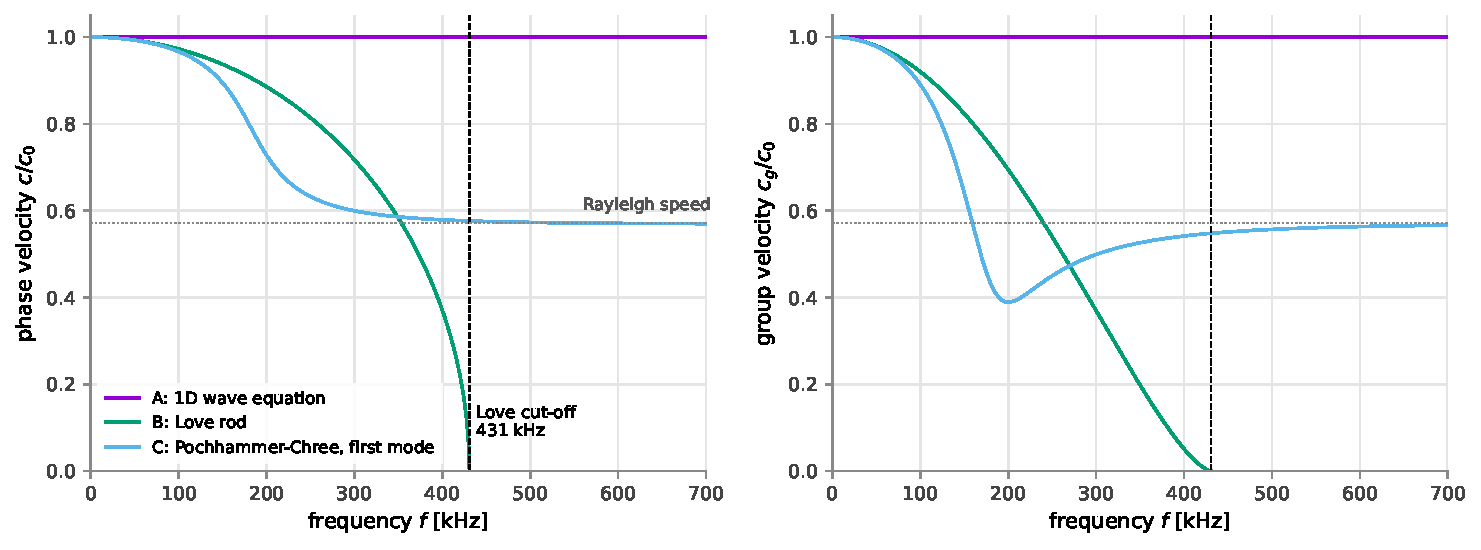
\includegraphics[width=\textwidth]{dispersion.pdf}
\caption{Phase velocity (left) and group velocity (right) relative to $c_0$ against frequency, for the aluminium
bar of the examples. A: one-dimensional wave equation; B: Love rod; C: first Pochhammer--Chree mode. Dashed
vertical line: the cut-off frequency of the Love rod, 431~kHz. Dotted horizontal line: the Rayleigh speed,
$c_R / c_0 = 0.571$. The curve of model B ends at its cut-off, above which the Love rod carries no propagating
wave.}
\label{fig:dispersion}
\end{figure}

\subsection{Model A: the one-dimensional wave equation}

The bar is treated as a line. Each cross-section moves only axially, and the stress is $E\varepsilon$:
\begin{equation}
  \rho\, u_{tt} = E\, u_{xx}, \qquad k = \frac{\omega}{c_0}.
\end{equation}
All frequencies travel at $c_0$, so a pulse keeps its shape. The model neglects the lateral motion of the bar,
which is caused by the Poisson effect. It is accurate for wavelengths much longer than the radius: in
\cref{tab:dispersion}, models B and C differ from it by less than 1\,\% below about 50~kHz.

\subsection{Model B: the Love rod}

Love added the kinetic energy of the lateral motion. An axial strain $\varepsilon$ contracts the cross-section by
$-\nu\varepsilon$, so a point at radius $r$ moves radially with velocity $-\nu r \dot\varepsilon$. The resulting
equation of motion is
\begin{equation}
  \rho\, u_{tt} = \frac{\partial}{\partial x}\Bigl[E\, u_x + \rho\, \nu^2 r_g^2\, u_{xtt}\Bigr], \qquad
  r_g^2 = \frac{a^2 + a_i^2}{2},
\end{equation}
where $r_g$ is the polar radius of gyration of the cross-section and $a_i$ the inner radius of a tube ($a_i = 0$
for a solid bar). For a wave $e^{i(\omega t - kx)}$ it gives the dispersion relation
\begin{equation}
  \frac{c^2}{c_0^2} = \frac{1}{1 + \nu^2 k^2 r_g^2}
  \quad\Longleftrightarrow\quad
  k^2 = \frac{\omega^2}{c_0^2 - \nu^2 r_g^2\, \omega^2}.
\end{equation}
The phase velocity decreases with frequency. For long waves it agrees with the Pochhammer--Chree solution to
leading order, $c / c_0 \approx 1 - \nu^2 (ka)^2 / 4$ for a solid bar, which a test confirms. At high frequency
the two models part (\cref{fig:dispersion}).

The Love rod has the cut-off frequency
\begin{equation}
  \omega_c = \frac{c_0}{\nu\, r_g}.
\end{equation}
At this frequency $k$ becomes infinite and the group velocity falls to zero. Above it, $k$ is imaginary, and the
wave does not propagate but decays with distance. For the example bar $f_c = 431$~kHz. This cut-off belongs to the
Love model, not to a real bar, whose first mode propagates at every frequency. The analysis therefore limits its
band to 0.8 times the cut-off when it uses this model.

\subsection{Model C: the first Pochhammer--Chree mode}

The Pochhammer--Chree solution~\cite{pochhammer1876, chree1889} treats the bar as a cylinder of linear elastic
material with a traction-free surface; it is the exact theory of harmonic longitudinal waves in an infinite
elastic rod~\cite{graff1975}. Axisymmetric solutions exist only if the frequency equation
\begin{equation}
  \frac{2\alpha}{a}(\beta^2 + k^2)\, J_1(\alpha a)\, J_1(\beta a)
  - (\beta^2 - k^2)^2\, J_0(\alpha a)\, J_1(\beta a)
  - 4 k^2 \alpha\beta\, J_1(\alpha a)\, J_0(\beta a) = 0
  \label{eq:pc}
\end{equation}
is satisfied, with
\begin{equation}
  \alpha^2 = \frac{\omega^2}{c_L^2} - k^2, \qquad \beta^2 = \frac{\omega^2}{c_T^2} - k^2.
\end{equation}
Here $J_0$ and $J_1$ are Bessel functions, and $c_L$ and $c_T$ are the longitudinal and shear wave speeds of the
material, related to $c_0$ by $c_0 / c_T = \sqrt{2(1 + \nu)}$. The equation has infinitely many branches (modes).
The simulator uses the first one, which starts at $c = c_0$ for long waves and approaches the Rayleigh
surface-wave speed $c_R$ for short waves. For the example bar $c_R / c_0 = 0.571$, the value approached in the last
rows of \cref{tab:dispersion}.

The function \code{pc_first_mode_table} solves \cref{eq:pc} once for each Poisson's ratio. It works in
dimensionless form, with the wavenumber $\xi = ka$ and the velocity $c / c_T$, and finds the lowest root above
$0.97\, c_R$ by bracketing and Brent's method on a grid of $\xi$ up to 100. The terms are scaled so that they stay
real when $\alpha$ or $\beta$ is imaginary. $k(\omega)$ is then interpolated from this table; beyond the table the
Rayleigh-speed asymptote is used. Tests compare the result with published roots for $\nu = 0.30$ and check both
limits.

The model is implemented for solid bars only. It contains only the first mode: near a bar end or the specimen, a
real bar also carries higher modes and non-propagating fields, which no single-mode model describes.

\subsection{The Kelvin--Voigt bar}

Models A and B can also be given a viscoelastic material: a spring $E$ in parallel with a dashpot of viscosity
$E\tau$. The stress is $\sigma = E(\varepsilon + \tau\dot\varepsilon)$, that is, the complex modulus
$E(1 + i\omega\tau)$, where $\tau$ is a retardation time. In the dispersion relation $c_0^2$ becomes
$c_0^2 (1 + i\omega\tau)$, so $k$ is complex with $\Imag k < 0$, and every component decays as it travels. For
$\omega\tau \ll 1$ and model A, the attenuation is $\omega^2\tau / (2c_0)$ and the phase velocity is
$c_0\bigl(1 + \tfrac{3}{8}(\omega\tau)^2\bigr)$. The model has one parameter, so it can match a real bar near one
frequency only; the README discusses its limits.

% =====================================================================================================
\section{The Bussac wave separation: the problem}
\label{sec:problem}

\begin{figure}[htbp]
\centering
\begin{tikzpicture}[x=1cm, y=1cm, >=stealth, font=\small]
  % bars and specimen (lengths not to scale)
  \fill[black!8] (0,-0.35) rectangle (6.6,0.35);
  \draw (0.4,-0.35) -- (6.6,-0.35) -- (6.6,0.35) -- (0.4,0.35);
  \draw[decorate, decoration={zigzag, amplitude=1.5pt, segment length=4pt}] (0.4,-0.35) -- (0.4,0.35);
  \fill[black!8] (7.4,-0.35) rectangle (14.0,0.35);
  \draw (14.0,-0.35) -- (7.4,-0.35) -- (7.4,0.35) -- (14.0,0.35);
  \draw[decorate, decoration={zigzag, amplitude=1.5pt, segment length=4pt}] (14.0,-0.35) -- (14.0,0.35);
  \fill[black!35] (6.6,-0.22) rectangle (7.4,0.22);
  \node at (3.5,0) {input bar};
  \node at (10.0,0) {output bar};
  \node at (7.0,0.62) {specimen};
  % strain gauges
  \foreach \g in {2.6, 5.1, 8.9, 11.4} \fill[black] (\g-0.12,0.35) rectangle (\g+0.12,0.45);
  % local coordinates: x = 0 at the interface, increasing into each bar
  \draw[->] (6.6,-1.25) -- (0.6,-1.25) node[below] {$x$};
  \draw[->] (7.4,-1.25) -- (13.8,-1.25) node[below] {$x$};
  \foreach \g/\l in {6.6/0, 5.1/x_1, 2.6/x_2, 7.4/0, 8.9/x_1, 11.4/x_2} {
    \draw (\g,-1.17) -- (\g,-1.33);
    \node[below] at (\g,-1.3) {$\l$};
    \draw[densely dotted, black!50] (\g,-1.17) -- (\g,-0.35);
  }
  % waves: P outgoing (away from the specimen), M incoming (towards it)
  \draw[->, very thick, color={rgb,255:red,0;green,158;blue,115}] (4.85,0.95) -- (2.35,0.95)
    node[midway, above] {$P$: outgoing, reflected wave $b_1$};
  \draw[->, very thick, color={rgb,255:red,148;green,0;blue,211}] (2.35,1.75) -- (4.85,1.75)
    node[midway, above] {$M$: incoming, incident wave $a_1$};
  \draw[->, very thick, color={rgb,255:red,0;green,158;blue,115}] (9.15,0.95) -- (11.65,0.95)
    node[midway, above] {$P$: outgoing, transmitted wave $b_2$};
  \draw[->, very thick, color={rgb,255:red,148;green,0;blue,211}] (11.65,1.75) -- (9.15,1.75)
    node[midway, above] {$M$: incoming, far-end echo $a_2$};
\end{tikzpicture}
\caption{Geometry of the separation. Each bar has its own local coordinate $x$, which is zero at the
bar--specimen interface and increases into the bar, so it points in opposite directions on the two bars. The
black marks are the strain gauges, at the distances $x_1$ and $x_2$ from the interface (0.30~m and 0.85~m in the
examples of \cref{sec:examples}). On each bar, $P$ is the wave that travels away from the specimen ($+x$) and $M$
the wave that travels towards it ($-x$); both are defined at $x = 0$. The labels name the same waves in the
notation of the simulator (\cref{sec:propagator}): $M = a$ and $P = b$. The far ends of the bars are not drawn,
and the lengths are not to scale.}
\label{fig:geometry}
\end{figure}

A gauge on a bar records the sum of the two waves that pass it. The separation has to recover, from the records of
one bar, the two waves at the interface; one bar is treated at a time. In the local coordinate $x \ge 0$, which
points from the interface into the bar, the two waves are $P$, the outgoing wave (\code{wave_out}), which leaves the
interface and travels in $+x$, and $M$, the incoming wave (\code{wave_in}), which travels in $-x$ towards the
interface. Both are defined at $x = 0$. \Cref{fig:geometry} shows the two waves on both bars. Because $x$ points
into each bar, the same equations hold for the input and the output bar.

The separation rests on one relation: how the spectrum of a wave at a gauge follows from its spectrum at the
interface. \Cref{sec:shift} derives this relation, first for the one-dimensional elastic bar and then for a
dispersive bar. \Cref{sec:gaugemodel} uses it to write the record of each gauge in terms of $P$ and $M$.

\subsection{Propagation as a time shift and as a phase factor}
\label{sec:shift}

\paragraph{The one-dimensional elastic bar.} In model A the axial displacement $u(x, t)$ obeys
$\rho\, u_{tt} = E\, u_{xx}$. Differentiating with respect to $x$ shows that the strain $\varepsilon = u_x$ obeys
the same wave equation, $\varepsilon_{tt} = c_0^2\, \varepsilon_{xx}$. Its general solution, due to d'Alembert, is
\begin{equation}
  \varepsilon(x, t) = P\!\left(t - \frac{x}{c_0}\right) + M\!\left(t + \frac{x}{c_0}\right),
  \label{eq:dalembert}
\end{equation}
where $P$ and $M$ are arbitrary functions of one variable. The first term has the same value wherever
$t - x / c_0$ is constant, that is, along $x = c_0 t + \text{const}$. It is therefore a wave that travels in the
$+x$ direction at the speed $c_0$ without changing shape: the outgoing wave. The second term travels in the $-x$
direction: the incoming wave. At the interface, $x = 0$, the two terms are $P(t)$ and $M(t)$, so the functions
$P$ and $M$ are exactly the time histories of the two waves at the interface.

At a gauge at the distance $x_j$, \cref{eq:dalembert} gives the two waves as
\begin{equation}
  \varepsilon_P(x_j, t) = P(t - \tau_j), \qquad \varepsilon_M(x_j, t) = M(t + \tau_j), \qquad
  \tau_j = \frac{x_j}{c_0}.
\end{equation}
The outgoing wave is delayed by the travel time $\tau_j$: it passes the gauge after it has left the interface.
The incoming wave is advanced by $\tau_j$: it passes the gauge before it reaches the interface.

\paragraph{The shift theorem.} With the transform of \cref{sec:notation},
$X(\omega) = \int x(t)\, e^{-i\omega t}\, dt$, a signal shifted in time by $\tau$ has the spectrum
\begin{equation}
  \int x(t - \tau)\, e^{-i\omega t}\, dt
  = \int x(t')\, e^{-i\omega (t' + \tau)}\, dt'
  = e^{-i\omega\tau}\, X(\omega),
  \label{eq:shift}
\end{equation}
with the substitution $t' = t - \tau$. A time shift therefore only multiplies each frequency component by a phase
factor, and leaves its amplitude unchanged. Applied to the two waves, with $\tau = +\tau_j$ for the outgoing and
$\tau = -\tau_j$ for the incoming wave, and with the wavenumber $k = \omega / c_0$ of model A, so that
$\omega\tau_j = k x_j$:
\begin{equation}
  \mathcal{F}[\varepsilon_P(x_j, \cdot)] = P(\omega)\, e^{-ikx_j}, \qquad
  \mathcal{F}[\varepsilon_M(x_j, \cdot)] = M(\omega)\, e^{+ikx_j}.
  \label{eq:shiftwaves}
\end{equation}
Here and below, $P(\omega)$ and $M(\omega)$ denote the spectra of the two waves at the interface. The factor
$e^{-ikx}$ of the outgoing wave is the propagator $H(\omega; x)$ of \cref{eq:propagator}, and the factor
$e^{+ikx}$ of the incoming wave is its inverse, $H(\omega; -x)$: propagation backwards in time over the same
distance.

The records are sampled, and the code uses the discrete Fourier transform. For it, \cref{eq:shift} holds exactly
only for a circular shift, in which samples pushed past the end of the record reappear at its start. This is why
the simulator pads the records with zeros (\cref{sec:propagator}), so that a delayed wave has room before the end
of the padded record instead of wrapping around.

\paragraph{A dispersive or damped bar.} For models B and C and for the Kelvin--Voigt bar, a pulse changes its shape
as it travels, and \cref{eq:dalembert} no longer holds. The bar is still linear and uniform along its length,
so each frequency component travels on its own as a harmonic wave $e^{i(\omega t - kx)}$, with the wavenumber
$k(\omega)$ given by the dispersion relation of the bar model (\cref{sec:models}). Because the bar is the same when
seen from either end, the dispersion relation contains only $k^2$, so $-k$ is also a solution: $e^{i(\omega t + kx)}$
is the same component travelling in $-x$. The spectra at the gauge are therefore again \cref{eq:shiftwaves}, now
with $k = k(\omega)$. The factor $e^{-ik(\omega)x} = e^{-i\omega x / c(\omega)}$ is a time shift of each component
by its own travel time $x / c(\omega)$, with the phase velocity $c(\omega) = \omega / k$. The components arrive at
different times, so the pulse changes shape. For a damped bar, $k$ is complex with $\Imag k < 0$, and the factor
also reduces the amplitude of each outgoing component by $e^{-\kappa x}$, with $\kappa = -\Imag k$; the incoming
component is correspondingly larger at the gauge, by $e^{+\kappa x}$, than when it reaches the interface. For
model A, $c(\omega) = c_0$ for every component, and the factor reduces to the single time shift of
\cref{eq:shift}.

\subsection{The records of the gauges}
\label{sec:gaugemodel}

A gauge at $x_j$ records the sum of the two waves, so by \cref{eq:shiftwaves} its spectrum is
$P\, e^{-ikx_j} + M\, e^{+ikx_j}$ for a gauge of zero length. Including the averaging over the gauge length, the
record $\hat\varepsilon_j$ of gauge $j$ is, at each frequency,
\begin{equation}
  \hat\varepsilon_j(\omega) = G_j(\omega)\Bigl[P(\omega)\, e^{-ik x_j} + M(\omega)\, e^{+ik x_j}\Bigr],
  \qquad j = 1, \dots, N.
  \label{eq:gaugemodel}
\end{equation}
Here $G_j(\omega)$ is the gauge factor of \cref{eq:gauge}, evaluated for the length $L_{g,j}$ of gauge $j$:
\begin{equation*}
  G_j(\omega) = \frac{\sin(k L_{g,j} / 2)}{k L_{g,j} / 2}.
\end{equation*}
It describes how the gauge records the strain averaged over its length, not the strain at its centre. It is the
same factor for both waves, because the average of $e^{\mp ikx}$ over a gauge centred at $x_j$ is
$G_j\, e^{\mp ikx_j}$ for either sign. For wavelengths much longer than the gauge it is close to 1,
$G_j \approx 1 - (k L_{g,j})^2 / 24$. For the 2~mm gauges of the examples on the Love rod it is 0.999 at 62~kHz,
0.997 at 100~kHz and 0.917 at the band limit of 345~kHz. In the separation, $G_j$ is evaluated with the continued
wavenumber $k(s)$ (\cref{sec:implementation}). The setting \code{gauge_length_correction = false} sets
$G_j = 1$, which treats each record as the strain at the gauge centre.

\Cref{eq:gaugemodel} is a linear relation between the records and the two unknowns, separately at each frequency. The separation
of Bussac, Collet, Gary and Othman~\cite{bussac2002} solves it frequency by frequency and transforms the result
back to the time domain.

% =====================================================================================================
\section{Two strain gauges}
\label{sec:twogauges}

With two gauges, and leaving out the gauge factors $G_j$ for clarity, there are two equations in two unknowns:
\begin{equation}
  \begin{pmatrix} e^{-ikx_1} & e^{+ikx_1} \\ e^{-ikx_2} & e^{+ikx_2} \end{pmatrix}
  \begin{pmatrix} P \\ M \end{pmatrix}
  =
  \begin{pmatrix} \hat\varepsilon_1 \\ \hat\varepsilon_2 \end{pmatrix}.
  \label{eq:twogauge}
\end{equation}
The determinant is
\begin{equation}
  D = e^{ik(x_2 - x_1)} - e^{-ik(x_2 - x_1)} = 2i \sin(k\Delta), \qquad \Delta = x_2 - x_1,
\end{equation}
and the solution is
\begin{equation}
  P = \frac{e^{+ikx_2}\, \hat\varepsilon_1 - e^{+ikx_1}\, \hat\varepsilon_2}{D}, \qquad
  M = \frac{e^{-ikx_1}\, \hat\varepsilon_2 - e^{-ikx_2}\, \hat\varepsilon_1}{D}.
  \label{eq:twogaugesolution}
\end{equation}

\subsection{The singular frequencies}

The solution fails where $D = 0$, that is, where $k\Delta = n\pi$ for $n = 0, 1, 2, \dots$. For a non-dispersive
bar these are the frequencies
\begin{equation}
  f_n = \frac{n\, c_0}{2\Delta}.
\end{equation}
At these frequencies the gauge spacing is a whole number of half wavelengths. A standing wave
$P e^{-ikx} + M e^{+ikx} \propto \sin\bigl(k(x - x_1)\bigr)$ then has nodes at both gauges: it produces no signal
at either gauge, so it cannot be detected, and any multiple of it can be added to the solution. At $n = 0$, zero
frequency, the same holds in another form: a constant strain can be divided between the two directions in any way.

For the example gauges at 0.30~m and 0.85~m on the aluminium bar, $\Delta = 0.55$~m, and the singular frequencies
are spaced by $c_0 / (2\Delta) = 4.6$~kHz. They lie throughout the band of a Hopkinson test. Near each of them $|D|$
is small, and the solution divides the records, together with any error in them, by a small number
(\cref{fig:conditioning}, left).

\begin{figure}[htbp]
\centering
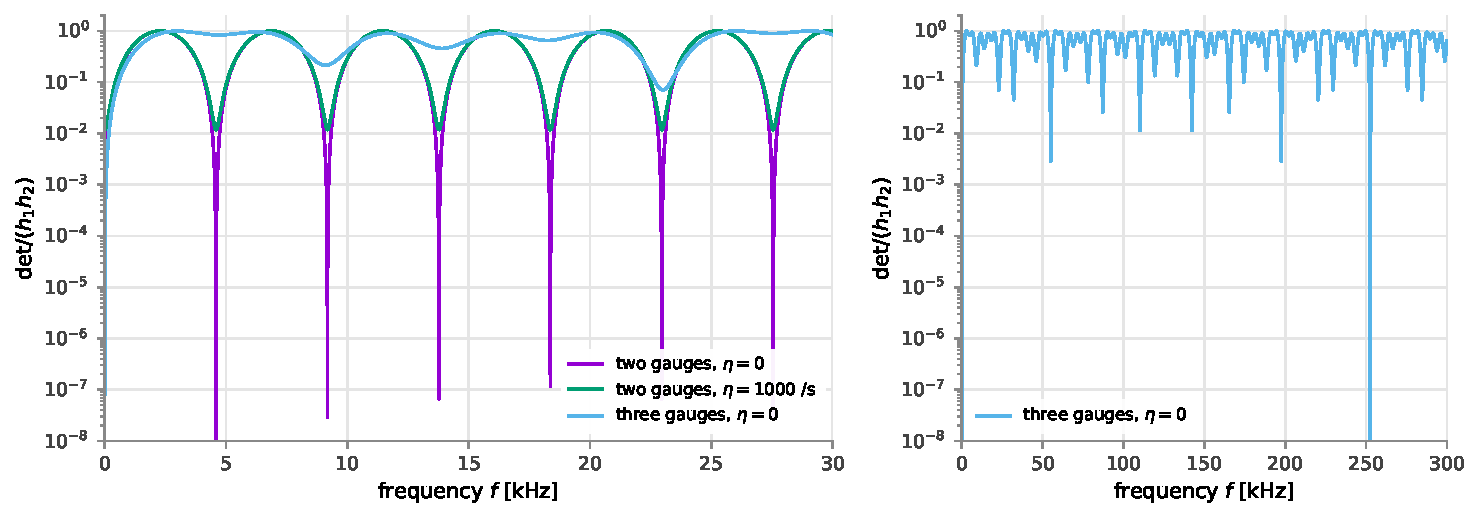
\includegraphics[width=\textwidth]{conditioning.pdf}
\caption{Normalised determinant $\det / (h_1 h_2)$ of the separation (\cref{sec:ngauges}) against frequency, for a
non-dispersive bar with the material of the examples and without gauge-length averaging. For two gauges it equals
$|D|^2 / (h_1 h_2)$; it is 1 where the two waves are best distinguished and 0 where they cannot be distinguished.
Values below $10^{-8}$ are drawn at $10^{-8}$. Left: two gauges at 0.30~m and 0.85~m without damping
($\eta = 0$) and with the Laplace damping $\eta = 1000$~/s, and three gauges at 0.30~m, 0.62~m and 0.85~m without
damping, up to 30~kHz. Right: the three gauges up to 300~kHz; their first singular frequency above zero is
252.6~kHz.}
\label{fig:conditioning}
\end{figure}

\subsection{The Laplace damping}

Bussac et al.\ avoid the singularities by evaluating the spectra at a complex frequency, $s = \omega - i\eta$ with
$\eta > 0$. This is the Laplace transform along a line parallel to the real axis. It is the same as multiplying the
records by $e^{-\eta t}$ before the Fourier transform, which is valid because the bar is at rest before the first
wave arrives. The wavenumber is continued analytically to $k(s)$ (\cref{sec:implementation}). For a non-dispersive
bar $k(s) = s / c_0$, and
\begin{equation}
  \bigl|\sin\bigl(k(s)\Delta\bigr)\bigr|^2
  = \sin^2\!\left(\frac{\omega\Delta}{c_0}\right) + \sinh^2\!\left(\frac{\eta\Delta}{c_0}\right),
\end{equation}
which never vanishes for $\eta > 0$. With $\eta = 1000$~/s and the example spacing, the smallest value of $|D|$ is
$2\sinh(\eta\Delta / c_0) = 0.22$, against a largest value of 2: at the worst frequency, errors are amplified about
ten times more than at the best. In \cref{fig:conditioning} the normalised determinant of the damped two-gauge
separation does not fall below 0.012.

The price is paid on the way back to the time domain, which multiplies by $e^{+\eta t}$. Errors in the separated
waves late in the record are amplified by this factor: by 2.7 after 1~ms and by 7.4 after 2~ms with
$\eta = 1000$~/s. A larger $\eta$ improves the conditioning at the singular frequencies and increases this late
amplification. The code refuses $\eta T > 700$, where $e^{\eta T}$ would overflow.

% =====================================================================================================
\section{N strain gauges: the least-squares solution}
\label{sec:ngauges}

With $N > 2$ gauges there are more equations than unknowns. With $\alpha_j = G_j e^{-ikx_j}$ and
$\beta_j = G_j e^{+ikx_j}$,
\begin{equation}
  \begin{pmatrix} \alpha_1 & \beta_1 \\ \vdots & \vdots \\ \alpha_N & \beta_N \end{pmatrix}
  \begin{pmatrix} P \\ M \end{pmatrix}
  \approx
  \begin{pmatrix} \hat\varepsilon_1 \\ \vdots \\ \hat\varepsilon_N \end{pmatrix}.
\end{equation}
Measured records contain noise, and an assumed bar model or gauge position is never exact. The $N$ equations are
then not satisfied by any single pair $(P, M)$. The separation chooses the pair that minimises the sum of the
squared residuals,
\begin{equation}
  S(P, M) = \sum_{j=1}^{N} \bigl|\hat\varepsilon_j - \alpha_j P - \beta_j M\bigr|^2.
  \label{eq:lsq}
\end{equation}
Setting the derivatives with respect to $P^*$ and $M^*$ to zero gives the normal equations
\begin{equation}
  \begin{pmatrix} h_1 & g \\ g^* & h_2 \end{pmatrix}
  \begin{pmatrix} P \\ M \end{pmatrix}
  =
  \begin{pmatrix} e_1 \\ e_2 \end{pmatrix},
  \label{eq:normal}
\end{equation}
with
\begin{equation}
  h_1 = \sum_j |\alpha_j|^2, \quad h_2 = \sum_j |\beta_j|^2, \quad g = \sum_j \alpha_j^* \beta_j, \quad
  e_1 = \sum_j \alpha_j^*\, \hat\varepsilon_j, \quad e_2 = \sum_j \beta_j^*\, \hat\varepsilon_j.
\end{equation}
Their solution is
\begin{equation}
  P = \frac{h_2\, e_1 - g\, e_2}{\det}, \qquad
  M = \frac{h_1\, e_2 - g^*\, e_1}{\det}, \qquad
  \det = h_1 h_2 - |g|^2.
\end{equation}
These are the formulas of the function \code{separate_spectra}.

\paragraph{Relation to the two-gauge case.} By the Cauchy--Schwarz inequality $\det \ge 0$, and by Lagrange's
identity
\begin{equation}
  \det = \sum_{j < l} \bigl|\alpha_j \beta_l - \alpha_l \beta_j\bigr|^2,
  \label{eq:lagrange}
\end{equation}
which is the sum of the squared two-gauge determinants of all pairs of gauges. For $N = 2$, $\det = |D|^2$, the
residual is zero, and the least-squares solution is the exact solution~\eqref{eq:twogaugesolution}.

For $N > 2$, $\det$ vanishes only if every pair of gauges is singular at the same frequency, that is, if every
spacing is a whole multiple of the same half wavelength. The singular frequencies of one pair are then covered by
the others. For the three gauges of \cref{fig:conditioning} the spacings are 0.23, 0.32 and 0.55~m. Their largest
common measure is 1~cm, so the first common singular frequency above zero is $c_0 / (2 \times 0.01~\mathrm{m})
= 252.6$~kHz, against 4.6~kHz for two gauges. Zero frequency remains singular for any number of gauges, which is
one reason the Laplace damping is still used. The code marks frequencies where $\det$ is below $10^{-14} h_1 h_2$
and sets the solution to zero there.

% =====================================================================================================
\section{The least-squares solution as the most likely solution}
\label{sec:likely}

Suppose the records differ from the model only by noise,
\begin{equation}
  \hat\varepsilon_j = \alpha_j P + \beta_j M + n_j,
\end{equation}
where the noise terms $n_j$ of the $N$ gauges are independent, have zero mean, and follow the same complex normal
distribution with variance $\sigma^2$. The probability of observing the records, for given $P$ and $M$, is then
\begin{equation}
  p(\hat\varepsilon_1, \dots, \hat\varepsilon_N \mid P, M) \propto \exp\!\left(-\frac{S(P, M)}{\sigma^2}\right).
\end{equation}
The pair $(P, M)$ that makes the observed records most probable is the pair that minimises $S$. The least-squares
solution is therefore the maximum-likelihood estimate of the two waves under this noise model. With a uniform
prior on $P$ and $M$, it is also the most probable pair given the records.

This interpretation gives three further results.

\paragraph{Uncertainty.} The covariance of the estimate is
\begin{equation}
  \cov(P, M) = \sigma^2 \begin{pmatrix} h_1 & g \\ g^* & h_2 \end{pmatrix}^{-1}.
\end{equation}
A small $\det$ therefore means a large uncertainty. The singular frequencies of \cref{sec:twogauges} are the
frequencies at which the records say little about the two waves, and more gauges reduce the uncertainty.

\paragraph{Without the normal distribution.} If the noise is only assumed to have zero mean, to be uncorrelated
and to have equal variance, but not to be normally distributed, the least-squares solution is still the linear
unbiased estimate with the smallest variance (Gauss--Markov theorem).

\paragraph{Conditions.} The interpretation holds only under its conditions, and three of them matter in practice.
\begin{itemize}
  \item \emph{Equal noise in every gauge.} The separation weights all gauges equally. If the gauges have different
  noise levels $\sigma_j$, the most likely solution weights each equation by $1 / \sigma_j^2$. This weighted form
  is not implemented.
  \item \emph{Errors are noise.} An error in the assumed wavenumber, gauge position or gauge length is not random.
  It biases the solution, and the least-squares solution is then the best fit of a wrong model, not the most likely
  true wave. The comparison of settings in the analysis exists to expose such differences on synthetic data.
  \item \emph{Each frequency on its own.} The solution is the most likely one at each frequency separately. The
  statement holds for the windowed spectra, in which the window $e^{-\eta t}$ weights early samples more than late
  ones. After windowing and zero padding, the noise of different frequency bins is no longer exactly independent.
\end{itemize}

% =====================================================================================================
\section{Details of the implementation}
\label{sec:implementation}

\paragraph{Continuation of the wavenumber.} The records are transformed at $s = \omega - i\eta$, so the propagation
factors must use $k(s)$, the analytic continuation of the dispersion relation. Using $s / c(\omega)$ instead would
damp each component with the phase velocity instead of approximately the group velocity, and gives an amplitude
error at dispersive frequencies. For model A, model B and the Kelvin--Voigt bar, the closed-form expressions are
evaluated at $s$; this is exact, and the principal square root is continuous with $\Imag k < 0$. For model C,
whose $k(\omega)$ is a table, a second-order Taylor expansion
$k(\omega) - i\eta\, k'(\omega) - \tfrac{1}{2}\eta^2 k''(\omega)$ is used.

\paragraph{Band limit.} Components above $f_\mathrm{max}$ are set to zero. Close to and above the Love cut-off the
Love model is not reliable, so the default band limit is 0.8 times the cut-off for model B. For a Kelvin--Voigt
bar the outgoing wave is damped on its way to the gauges, so its reconstruction at the interface multiplies by
$e^{+\kappa x}$; the band is limited further, to keep this factor below $10^3$ at the farthest gauge.

\paragraph{Interface quantities.} From $P$ and $M$ at the interface the analysis forms the strain $P + M$, the
velocity with the operator $\mp s / k$ of each wave, and the forces $A E (P + M)$ and $A\rho(s / k)^2 (P + M)$. All
of these are formed in the Laplace domain, before the inverse transform, which multiplies by $e^{+\eta t}$.

\paragraph{Valid window.} The outgoing wave at the interface at time $t$ reaches the farthest gauge, at
$x_\mathrm{max}$, only at about $t + x_\mathrm{max} / c_0$. The separated waves are therefore compared with the
truth only for $t < T - x_\mathrm{max} / c_0 - t_\mathrm{margin}$, where $T$ is the end of the record and
$t_\mathrm{margin}$ the setting \code{valid_margin}.

% =====================================================================================================
\section{Worked examples}
\label{sec:examples}

This section applies both programs to two example cases of the project, a split Hopkinson pressure bar (SHPB) and
a split Hopkinson tension bar (SHTB). In each, the simulator produces the gauge records and the true interface
waves, and the analysis separates the records with exactly the settings of the simulation: the same bar model, bar
material, gauge positions and gauge length. The examples therefore show how the method behaves when its
assumptions are met. They do not show the effect of a wrong bar model or a wrong gauge position, and they contain
no measurement noise.

\subsection{What is shown and how the errors are measured}

For each example, two figures are shown. The first shows the simulated gauge records of both bars, which are the
only input of the analysis, and the separated waves at the two interfaces drawn over the simulated (true) waves.
The second shows the interface forces $N_1$ of the input bar and $N_2$ of the output bar, both computed as
$N = A E (a + b)$ from the separated waves, together with the true forces, and their relative imbalance
\begin{equation}
  r(t) = \frac{N_1 - N_2}{N_m}, \qquad N_m = \tfrac{1}{2}(N_1 + N_2).
\end{equation}
The imbalance is evaluated only where $|N_m|$ is at least 5\,\% of its peak in the valid window, because the ratio
has no meaning while both forces are close to zero. This is the check of specimen equilibrium that the analysis
draws in its second window: in a valid test, the specimen is loaded almost equally from both sides, and $r$ stays
small after the first rise of the force.

In both examples the specimen is the lumped model of the simulator, in which the stress is uniform along the
specimen at every instant. The true forces are therefore equal by construction, and the true imbalance is zero
to the printed digits. The force-balance figures thus show how far the separation alone creates an apparent
imbalance; they say nothing about whether a real specimen would reach equilibrium.

The separation is valid only up to the time $t_v = T - x_\mathrm{max} / c_0 - t_\mathrm{margin}$
(\cref{sec:implementation}), with the farthest gauge at $x_\mathrm{max} = 0.85$~m and $t_\mathrm{margin} = 20~\mu$s.
After $t_v$ the figures are shaded grey, and no error is evaluated there. The error of a separated wave is its
largest absolute difference from the true wave in the valid window, divided by the peak of the true incident wave
$a_1$; the error of a force is divided in the same way by the peak of the true input-bar force. The quoted wave
error is the largest of the four waves, and the quoted force error the larger of the two forces.

\subsection{Split Hopkinson pressure bar}

\paragraph{Setup.} Both bars are aluminium (Al~7075: $E = 71.7$~GPa, $\rho = 2810~\mathrm{kg/m^3}$, $\nu = 0.33$),
2~m long and 16~mm in diameter, and are described by the Love rod (model B). Each bar has two gauges of 2~mm length,
at 0.30~m and 0.85~m from the interface. A compressive strain pulse of amplitude $10^{-3}$ is prescribed at the far
end of the input bar, 2~m from the interface; it rises in 4~\textmu{}s, holds for 150~\textmu{}s and falls in
10~\textmu{}s. The specimen is a commercially pure aluminium cylinder, 5~mm long and 10~mm in diameter,
elastic--plastic with linear hardening and a logarithmic strain-rate dependence, in unilateral contact with the bars.
The records are sampled at 5~MHz for 1~ms. The analysis uses $\eta = 1000$~/s and the band limit
$f_\mathrm{max} = \shpbFmax$~kHz, which is 0.8 times the Love cut-off of the bars.

\paragraph{Signals.} \Cref{fig:shpb-signals} shows the records and the separated waves. The incident wave reaches the
interface at about 415~\textmu{}s. Because of the dispersion of the Love rod, the short rise of the pulse becomes a
front followed by oscillations, which grow with the distance travelled. The reflected wave in the input bar is
tensile: the specimen, with a smaller cross-section than the bar and yielding early, carries less force than a
continuation of the bar would. The transmitted wave has the shape of the
specimen force, rising as the specimen hardens and ending when the incident pulse ends. The far-end echo of the
output bar would return to the interface after the end of the record, so $a_2$ is zero. The separated waves agree
with the true waves within the line width in the valid window, which ends at $t_v = \shpbValid$~\textmu{}s.

\begin{figure}[htbp]
\centering
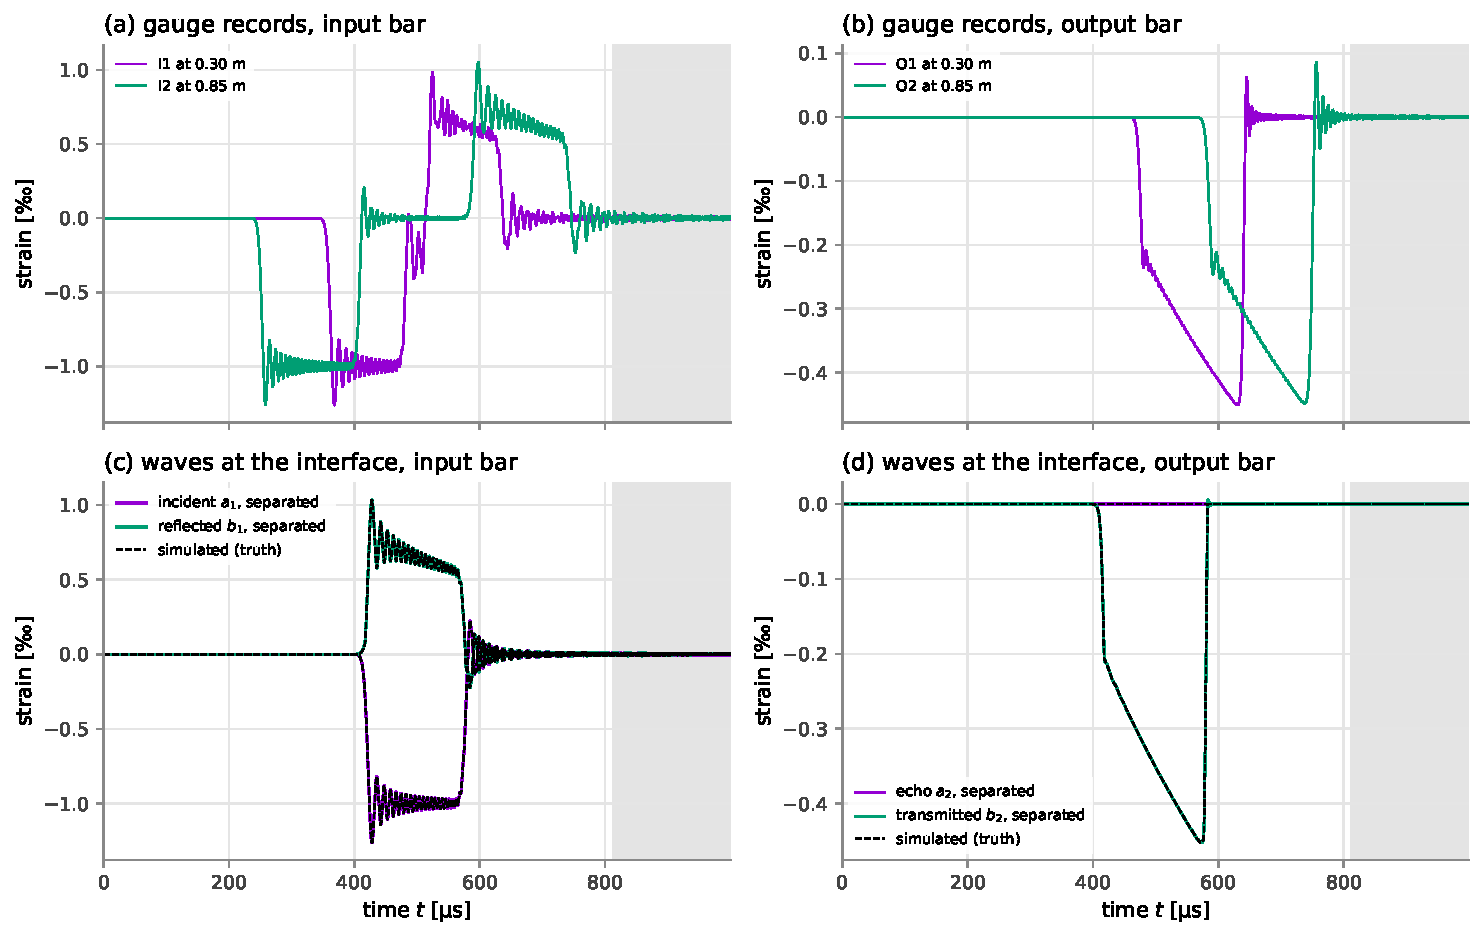
\includegraphics[width=\textwidth]{SHPB_signals.pdf}
\caption{SHPB example. (a), (b): simulated gauge records of the input and the output bar; I1, I2 are the gauges on
the input bar and O1, O2 those on the output bar, at the stated distances from the interface. They are averaged
over the gauge length. (c), (d): waves at the interface, separated from the records (coloured lines) and simulated
(black dashed lines). $a_1$ and $b_1$ are the incident and the reflected wave of the input bar; $a_2$ is the
incoming wave of the output bar, its far-end echo, and $b_2$ the transmitted wave. Strain in units of $10^{-3}$,
tension positive. Grey: outside the valid window of the separation.}
\label{fig:shpb-signals}
\end{figure}

\paragraph{Errors.} In the valid window the largest wave error is $\shpbWaveErr$ and the largest force error
$\shpbForceErr$, both relative to the peak of the incident wave or force. Most of the wave error comes from the band
limit: the separated waves contain no frequencies above $f_\mathrm{max}$, while the true waves of a pulse with a
4~\textmu{}s rise do. Compared with the true waves limited to the same band, in the same way as in the analysis,
the largest wave error falls to $1.2 \cdot 10^{-3}$. The remaining error lies in the last few tens of microseconds of
the valid window, in the reflected wave; before $t_v - 200~\mu$s it is below $3 \cdot 10^{-5}$. This agrees with the
factor $e^{+\eta t}$ of the inverse transform, which amplifies errors most at late times (\cref{sec:twogauges}).
The cause of the small error that is amplified there was not investigated.

\paragraph{Force balance.} \Cref{fig:shpb-forces} shows the two separated interface forces, which cannot be
distinguished at the scale of the figure. The largest relative imbalance of the separated forces is
$\shpbImbSep$~\%, against $\shpbImbTrue$~\% for the true forces.

\begin{figure}[htbp]
\centering
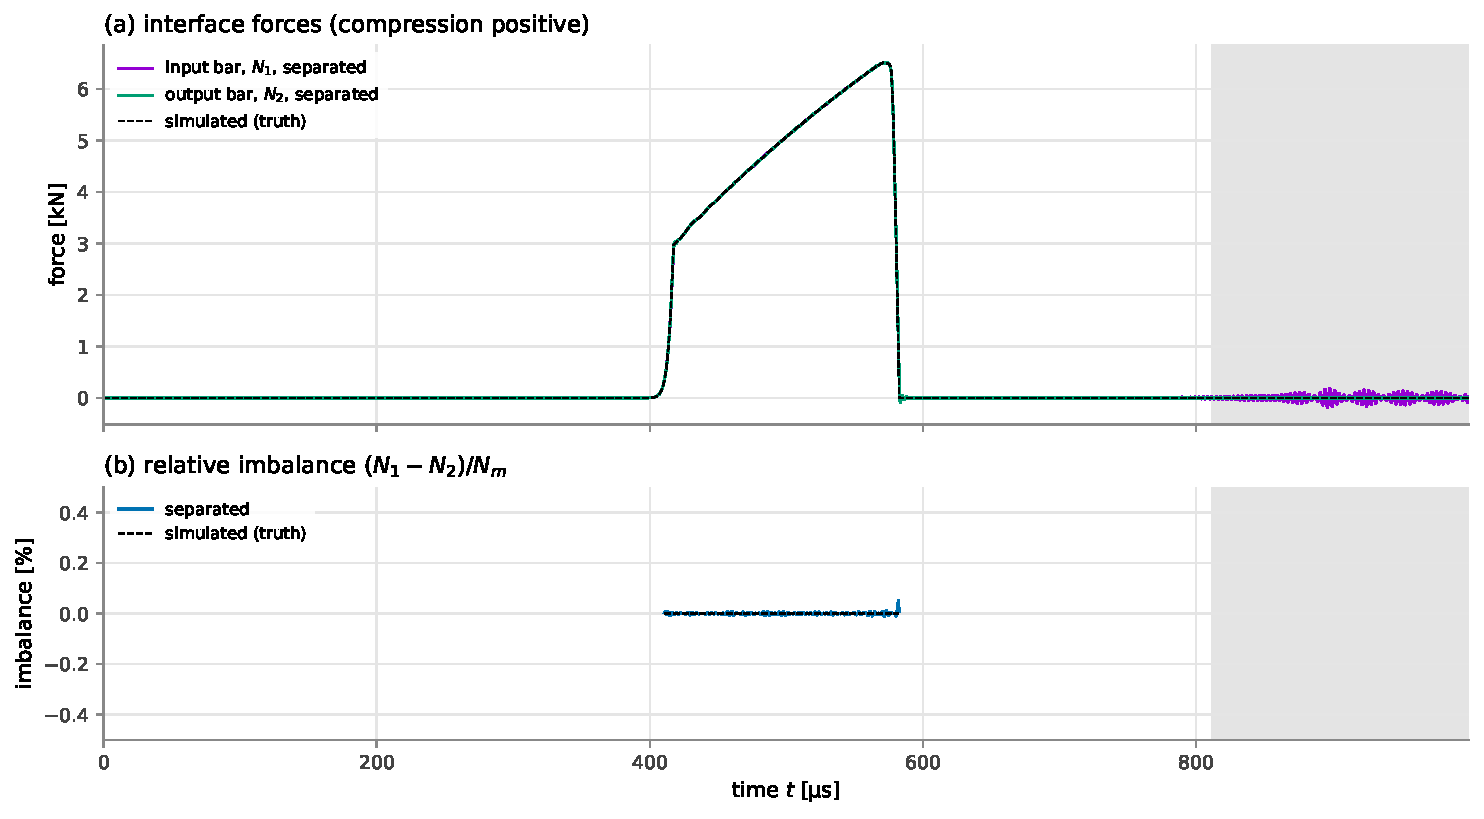
\includegraphics[width=\textwidth]{SHPB_forces.pdf}
\caption{SHPB example, force balance of the specimen. (a): interface forces $N_1$ (input bar) and $N_2$ (output
bar), $N = AE(a + b)$, from the separated waves (coloured lines) and from the simulated waves (black dashed lines),
compression positive. (b): relative imbalance $(N_1 - N_2)/N_m$ with $N_m = (N_1 + N_2)/2$, drawn only where
$|N_m|$ is at least 5\,\% of its peak in the valid window. Grey: outside the valid window.}
\label{fig:shpb-forces}
\end{figure}

\subsection{Split Hopkinson tension bar}

\paragraph{Setup.} Both bars are of the same aluminium as in the SHPB example, 16~mm in diameter and 2.7~m long, and
are described by the Love rod. The gauges are again at 0.30~m and 0.85~m from the interface. A tubular striker of
polyoxymethylene (outer diameter 40~mm, inner diameter 16~mm, 0.8~m long) slides over the input bar and hits a
steel flange of 0.197~kg at its far end at 5~m/s, which sends a tensile pulse of about 1.1~ms into the input bar.
The specimen is a commercially pure aluminium cylinder, 10~mm long and 4~mm in diameter, bonded to both bars, with
the same material model as in the SHPB example. The records are sampled at 5~MHz for 2~ms. The analysis uses the
same $\eta$ and the band limit $f_\mathrm{max} = \shtbFmax$~kHz.

\paragraph{Signals.} \Cref{fig:shtb-signals} shows the records and the separated waves. The incident pulse reaches
the interface at about 555~\textmu{}s. Its rise is slower than in the SHPB example, because it is shaped by the
contact of the striker with the flange, so the oscillations of dispersion are much smaller. The specimen is far
thinner than the bars, so most of the incident wave is reflected, and the transmitted wave is small. At about
1620~\textmu{}s, one round trip of $2 \times 2.7$~m after the arrival of the incident pulse, the echoes of the
flange and of the free end of the output bar reach the interface: the reflected wave $b_1$ returns in $a_1$, and the
transmitted wave $b_2$ returns with the opposite sign in $a_2$. The separation follows these echoes as well as the
first waves. The valid window ends at $t_v = \shtbValid$~\textmu{}s.

\begin{figure}[htbp]
\centering
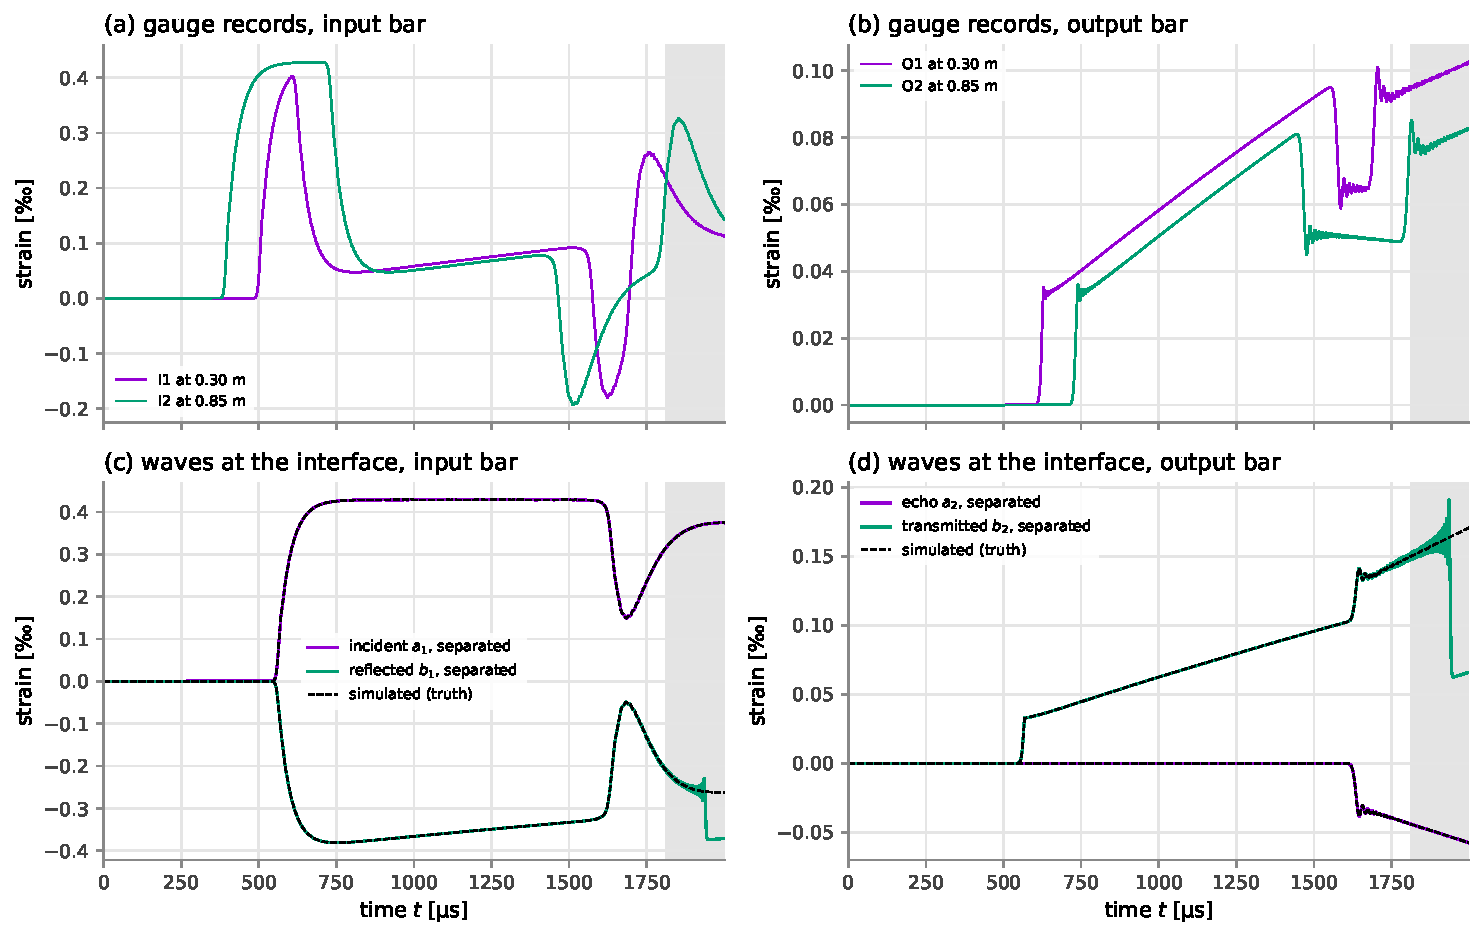
\includegraphics[width=\textwidth]{SHTB_signals.pdf}
\caption{SHTB example. (a), (b): simulated gauge records of the input and the output bar, averaged over the gauge
length; I1, I2 and O1, O2 as in \cref{fig:shpb-signals}. (c), (d): waves at the interface, separated from the
records (coloured lines) and simulated (black dashed lines); $a_1$, $b_1$, $a_2$, $b_2$ as in
\cref{fig:shpb-signals}. Strain in units of $10^{-3}$, tension positive. Grey: outside the valid window of the
separation.}
\label{fig:shtb-signals}
\end{figure}

\paragraph{Errors.} In the valid window the largest wave error is $\shtbWaveErr$ and the largest force error
$\shtbForceErr$. Here the band limit is not the cause: compared with the true waves limited to the same band, the
largest wave error is $6.3 \cdot 10^{-3}$, about the same. As in the SHPB example, the error is largest at the end of
the valid window, in the outgoing waves of both bars; before $t_v - 200~\mu$s it is below $5.4 \cdot 10^{-4}$. The
oscillation of the transmitted wave in \cref{fig:shtb-signals}(d), which grows from about 1700~\textmu{}s on, is
this error. The record of this example is 2~ms long, so the factor $e^{+\eta t}$ reaches 6 at the end of the valid
window, against 2.3 in the SHPB example. Whether this factor explains the larger error was not tested, for example
by repeating the separation with a smaller $\eta$.

\paragraph{Force balance.} \Cref{fig:shtb-forces} shows the two separated interface forces and their imbalance. The
largest relative imbalance of the separated forces is $\shtbImbSep$~\%, against $\shtbImbTrue$~\% for the true
forces. The imbalance stays below 0.04\,\% until about 1650~\textmu{}s and then grows towards the end of the valid
window, where the separated waves have their largest error.

\begin{figure}[htbp]
\centering
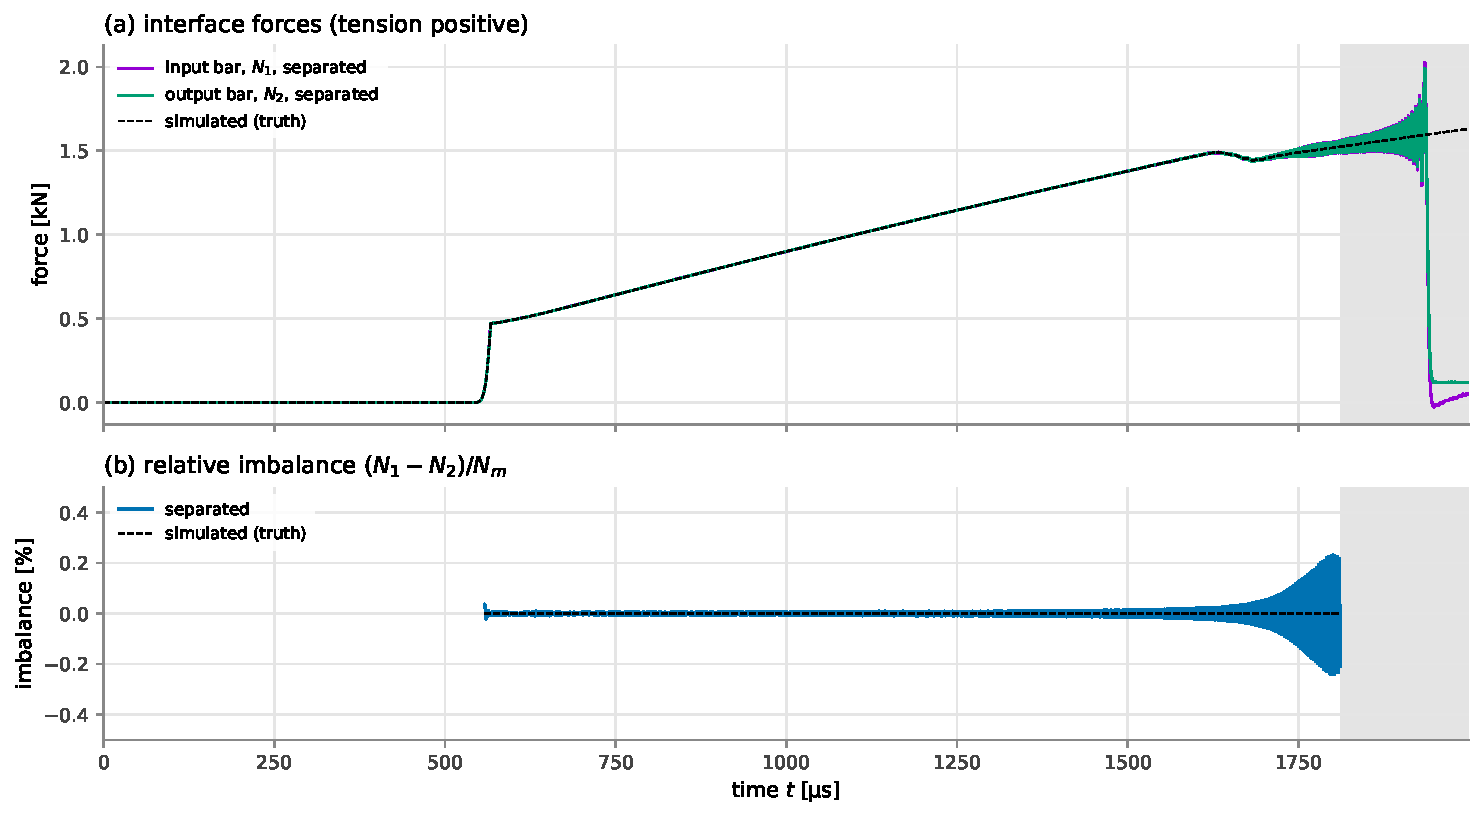
\includegraphics[width=\textwidth]{SHTB_forces.pdf}
\caption{SHTB example, force balance of the specimen. (a): interface forces $N_1$ (input bar) and $N_2$ (output
bar), $N = AE(a + b)$, from the separated waves (coloured lines) and from the simulated waves (black dashed lines),
tension positive. (b): relative imbalance $(N_1 - N_2)/N_m$, drawn only where $|N_m|$ is at least 5\,\% of its peak
in the valid window. Grey: outside the valid window.}
\label{fig:shtb-forces}
\end{figure}

\subsection{What the examples show}

In both examples the separation recovers the four interface waves from the two records of each bar to about
$10^{-2}$ of the incident peak or better, and the separated forces show the equilibrium of the specimen to a few
tenths of a percent. Both statements hold for exact records and a correct bar model; the errors stated above are
those of the method with its band limit and its finite record, not those of a measurement. Each example is one run,
with one value of $\eta$ and one band limit. The examples do not show how the errors change with noise in the
records, with a wrong bar model, or with a wrong gauge position. The analysis program can study the last two by
changing its case file (\cref{sec:likely}).

% =====================================================================================================
\appendix
\section{Reproduction}
\label{sec:reproduction}

The methods are implemented in \code{hopkinson_simulator.py} (bar models, propagation, specimen, the three setups)
and \code{bussac_analysis.py} (the separation) in the root of the project; the tests in \code{tests/} check the
statements that this report attributes to a test. The numbers of \cref{tab:dispersion} and the values quoted in
\cref{sec:twogauges,sec:ngauges} were computed with these two files. The figures, and the numbers quoted in \cref{sec:examples}, are made by
\code{reports/theory/make_figures.py}, which imports the same code. For the worked examples it runs the
simulation cases \code{simulation_cases/SHPB.toml} and \code{simulation_cases/SHTB.toml} and the analysis cases
of the same names in \code{analysis_cases/}, with the functions the two programs use, but in memory: it does not
write and read the records file, whose 12 significant digits change none of the quoted numbers. It stops if an
analysis case differs from its simulation case. It writes the numbers to \code{figures/examples.tex}, which this
report reads. The PDF is built with \code{make} in
\code{reports/theory/}; its title page names the commit of the source.

\begin{thebibliography}{9}
\bibitem{bussac2002}
M.-N. Bussac, P.~Collet, G.~Gary, R.~Othman.
\newblock An optimisation method for separating and rebuilding one-dimensional dispersive waves from multi-point
measurements. Application to elastic or viscoelastic bars.
\newblock \emph{Journal of the Mechanics and Physics of Solids}, 50:321--349, 2002.

\bibitem{chree1889}
C.~Chree.
\newblock \emph{Transactions of the Cambridge Philosophical Society}, 14, 1889. (The frequency equation of the
elastic cylinder, found independently of Pochhammer.)

\bibitem{graff1975}
K.~F. Graff.
\newblock \emph{Wave Motion in Elastic Solids}.
\newblock Oxford University Press, 1975.

\bibitem{love1927}
A.~E.~H. Love.
\newblock \emph{A Treatise on the Mathematical Theory of Elasticity}, 4th edition.
\newblock Cambridge University Press, 1927.

\bibitem{pochhammer1876}
L.~Pochhammer.
\newblock Ueber die Fortpflanzungsgeschwindigkeiten kleiner Schwingungen in einem unbegrenzten isotropen
Kreiscylinder.
\newblock \emph{Journal für die reine und angewandte Mathematik}, 81, 1876.
\end{thebibliography}

\end{document}
